\documentclass[12pt, a4paper]{report}
%\documentclass[11pt, a4paper]{article}

%====================== PACKAGES ======================
\usepackage[french]{babel}

\frenchbsetup{StandardLists=true}
\usepackage{enumitem}
\usepackage{pifont}

\usepackage[utf8x]{inputenc}
%\usepackage[latin1]{inputenc}

%pour gérer les positionnement d'images
\usepackage{float}
\usepackage{amsmath}
\DeclareMathOperator{\dt}{dt}
\usepackage{graphicx}
%\usepackage{tabularx}
\usepackage[colorinlistoftodos]{todonotes}
\usepackage{url}

%pour les informations sur un document compilé en PDF et les liens externes / internes
\usepackage[pdfborder=0]{hyperref}
\hypersetup{
	colorlinks = true
	}

%pour la mise en page des tableaux
\usepackage{array}
\usepackage{tabularx}
\usepackage{multirow}
\usepackage{multicol}
\setlength{\columnsep}{50pt}

%pour utiliser \floatbarrier
%\usepackage{placeins}
%\usepackage{floatrow}

%espacement entre les lignes
\usepackage{setspace}

%modifier la mise en page de l'abstract
\usepackage{abstract}

%police et mise en page (marges) du document
\usepackage[T1]{fontenc}
\usepackage[top=2cm, bottom=2cm, left=2cm, right=2cm]{geometry}

%Pour les galerie d'images
\usepackage{subfig}

\usepackage{pdfpages}

\usepackage{tikz}
\usetikzlibrary{trees}
\usetikzlibrary{decorations.pathmorphing}
\usetikzlibrary{decorations.markings}
\usetikzlibrary{decorations.pathreplacing,calligraphy}
%\usetikzlibrary{decorations}
\usetikzlibrary{angles, quotes}
\usepackage{verbatim}

\usepackage{appendix}

\usepackage{comment}

\usepackage{xcolor}

%\PreviewEnvironment{tikzpicture}
%\setlength\PreviewBorder{0pt}%

%====================== INFORMATION ET REGLES ======================

%rajouter les numérotation pour les \paragraphe et \subparagraphe
\setcounter{secnumdepth}{4}
\setcounter{tocdepth}{4}

\hypersetup{							% Information sur le document
pdfauthor = {Stephan Runigo},			% Auteurs
pdftitle = {Documentation},			% Titre du document
pdfsubject = {Documentation},		% Sujet
pdfkeywords = {Document},	% Mots-clefs
pdfstartview={FitH}}	% ajuste la page à la largeur de l'écran
%pdfcreator = {MikTeX},% Logiciel qui a crée le document
%pdfproducer = {} % Société avec produit le logiciel

%======================== DEBUT DU DOCUMENT ========================
%
\begin{document}
%
%régler l'espacement entre les lignes
\newcommand{\HRule}{\rule{\linewidth}{0.5mm}}
%
% Titre, résumé, ... %
%
\begin{titlepage}
%
~\\[1cm]

\begin{center}
%\includegraphics[scale=0.5]{./presentation/chambreABulle}
\end{center}

\textsc{\Large }\\[0.5cm]

% Title \\[0.4cm]
\HRule

\begin{center}
{\huge \bfseries  La causalité\\
%titre 2\\[0.4cm]
 }
\end{center}

\HRule \\[1.5cm]

\begin{center}
%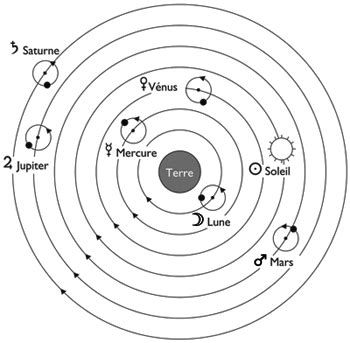
\includegraphics[scale=0.3]{./presentation/ptoleme}
\end{center}

\begin{center}
%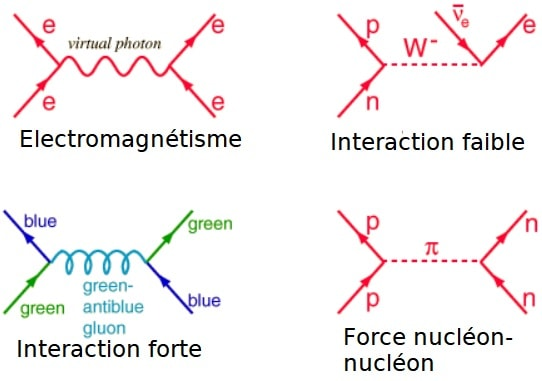
\includegraphics[scale=0.3]{./presentation/diagrammesInteractions}
\end{center}


% Author and supervisor
\begin{minipage}{0.4\textwidth}
\begin{flushleft} \large
%\emph{Auteur:}\\
%Stephan \textsc{Runigo}
\end{flushleft}
\end{minipage}
\begin{minipage}{0.4\textwidth}
\begin{flushright} \large
\emph{Auteur:}\\
Stephan \textsc{Runigo}
\end{flushright}
\end{minipage}

\vfill

% Bottom of the page
{\large \today}

\end{titlepage}

\newpage
\begin{center}
\Large
Résumé
\normalsize
\end{center}
\vspace{3cm}
\begin{itemize}[leftmargin=1cm, label=\ding{32}, itemsep=21pt]
\item {\bf Objet : } Souvenir des questions posés.
\item {\bf Contenu : } Définition, analyse, reflexion.
\item {\bf Public concerné : } Interressé à la question de l'âme.
\end{itemize}

\vspace{3cm}



\vspace{3cm}


%

%
% Table des matières
\tableofcontents
\thispagestyle{empty}
\setcounter{page}{0}
%
%espacement entre les lignes des tableaux
\renewcommand{\arraystretch}{1.5}
%
%====================== INCLUSION DES CHAPITRES ======================
%
~
\thispagestyle{empty}
%recommencer la numérotation des pages à "1"
\setcounter{page}{0}
\newpage
%
\chapter{Le vocabulaire des physiciens}
%
\section{Introduction}

Lorsque des scientifiques découvrent quelque chose de nouveau, ils le nomment. Le nom choisi peut être un nom propre, hommage ou clin d'œuil au découvreur ou à l'un des précursseur à 

%
\section{Masse}

\subsection{Grandeur et système}
La physique moderne distingue les grandeurs et les systèmes : un {\bf système} est un ensemble de corps matériel, auquel on associe des {\bf grandeurs}, caractéristiques du système.

\subsection{Masse et corps matériel}
La masse est une grandeur physique. Elle s'exprime en kg et se mesure à l'aide de balance. 

\subsection{La confusion}
Dans un certain nombre d'écrit (concernant la physique), on appelle {\it masse} le corps constituant une partie du système physique (masse du pendule, de l'oscillateur...) qui possède une masse.

Ainsi, dans ces écrits, on confond une partie du système avec une grandeur, on appelle {\it masse} un corps.

\subsection{Le pendule pesant}
Un pendule est constitué d'une masse suspendu


%
\section{Le temps}

Les équations de newton font intervenir une variable. Newton appelera cette variable {\it temps}, concept existant se rapprochant le plus (pour Newton) de la variable introduite dans les équations.

%
\chapter{Formulaire}
\subsection{Mécanique analytique}

Action S et lagrangien L

Principe

\[
S = \int_{t_1}^{t_2} L(q_i, \dot{q}_i, t)dt \ \ \ \ \ \ \text{est extrémale}
\]

L'invariance du lagrangien par translation temporelle entraine le théorème :

\[
E \ \text{est une constante du mouvement}
\]

\subsection{Thermodynamique}

Énergie U, entropie S, température T, chaleur Q, travail W,  pression P, volume V

Principes
\[
dU = \delta Q + \delta W \ \ \ \ \ \ dS = \frac{\delta Q}{T}
\]
Théorème TdS
\[
dU = TdS - pdV
\]

\subsection{Quantique}
L'énergie est une observable, dans un système isolé,
\[
\mc{H}|\psi(x,t)\rangle=E|\psi(x,t)\rangle
\]


\[
\mc{H} = -i\hbar\frac{\partial}{\partial t} \ \ \ \ \ \ \ \mc{P} = i\hbar\frac{\partial}{\partial x}
\]

%

%
%
%%\section{B}
\chapter{}
%%{\bf }{\it }{\bf --} « » {\footnotesize X}$^\text{e}$
\section{Bigbang}

Lors des premiers instants du bigbang l'expansion de l'univers se serait produite à des vitesses supérieur à celle de la lumière.
Quelques instants plus tard, une transition de phase se serait produite transformant l'univers primordiale en un univers constitué de photon et d'autre particules.
Certaine de ces particule ayant une masse.
Cette transition de phase (ou une autre ?) aurait produit la masse en plus de fixer une vitesse limite.





{\footnotesize
\begin{itemize}[leftmargin=1cm, label=\ding{32}, itemsep=1pt]
\item {\bf \textsc{Étymologie} :} latin {\it },.
\item {\bf \textsc{Sens ordinaire} :} .
\item {\bf \textsc{Spiritualisme} :} .
\end{itemize}

\begin{itemize}[leftmargin=1cm, label=\ding{32}, itemsep=1pt]
\item {\bf \textsc{Terme voisin} :} .
\item {\bf \textsc{Terme opposé} :} .
\item {\bf \textsc{Corrélats} :} .
\end{itemize}
}

%%%%%%%%%%%%%%%%%%%
\section{}
%%%%%%%%%%%%%%%%%%%
{\footnotesize
\begin{itemize}[leftmargin=1cm, label=\ding{32}, itemsep=1pt]
\item {\bf \textsc{Étymologie} :} latin {\it },.
\item {\bf \textsc{Sens ordinaire} :} .
\item {\bf \textsc{Terme voisin} :} .
\item {\bf \textsc{Terme opposé} :} .
\item {\bf \textsc{Corrélats} :} .
\end{itemize}
}

\chapter{A}
%%{\bf }{\it }{\bf --}{\footnotesize X}$^\text{e}$
\section{Analogie}





\subsection{Incertitude}

Sécuriser son territoire, réduire l'incertitude, prendre une assurance,
car il y aurait un principe d'incertitude macroscopique.
Par analogie, on utilise abusivement ce terme en physique quantique

\subsection{Vibration}

Chronologiquement, l'Homme découvre le phénomène de la vibration.
Puis le caractère vibratoire au niveau quantique. Ce n'est pas parceque
la matière est fondamentalement vibratoire mais c'est parceque notre
entendement ne nous permet pas de comprendre la quantique. Notre
entendement nous mermet de distinguer le granulaire de l'ondulatoire.
Ni le granulaire ni l'ondulatoire ne sont vrai, la réalité est autre.
Si la théorie quantique parle d'onde et de corpuscule, c'est parceque
nous n'avons pas les capacités d'aller plus loin






{\footnotesize
\begin{itemize}[leftmargin=1cm, label=\ding{32}, itemsep=1pt]
\item {\bf \textsc{Étymologie} :} latin {\it },.
\item {\bf \textsc{Sens ordinaire} :} .
\item {\bf \textsc{Spiritualisme} :} .
\end{itemize}

\begin{itemize}[leftmargin=1cm, label=\ding{32}, itemsep=1pt]
\item {\bf \textsc{Terme voisin} :} .
\item {\bf \textsc{Terme opposé} :} .
\item {\bf \textsc{Corrélats} :} .
\end{itemize}
}

%\chapter{}
%%{\bf }{\it }{\bf --} « » {\footnotesize X}$^\text{e}$
\section{Bigbang}

Lors des premiers instants du bigbang l'expansion de l'univers se serait produite à des vitesses supérieur à celle de la lumière.
Quelques instants plus tard, une transition de phase se serait produite transformant l'univers primordiale en un univers constitué de photon et d'autre particules.
Certaine de ces particule ayant une masse.
Cette transition de phase (ou une autre ?) aurait produit la masse en plus de fixer une vitesse limite.





{\footnotesize
\begin{itemize}[leftmargin=1cm, label=\ding{32}, itemsep=1pt]
\item {\bf \textsc{Étymologie} :} latin {\it },.
\item {\bf \textsc{Sens ordinaire} :} .
\item {\bf \textsc{Spiritualisme} :} .
\end{itemize}

\begin{itemize}[leftmargin=1cm, label=\ding{32}, itemsep=1pt]
\item {\bf \textsc{Terme voisin} :} .
\item {\bf \textsc{Terme opposé} :} .
\item {\bf \textsc{Corrélats} :} .
\end{itemize}
}

%%%%%%%%%%%%%%%%%%%
\section{}
%%%%%%%%%%%%%%%%%%%
{\footnotesize
\begin{itemize}[leftmargin=1cm, label=\ding{32}, itemsep=1pt]
\item {\bf \textsc{Étymologie} :} latin {\it },.
\item {\bf \textsc{Sens ordinaire} :} .
\item {\bf \textsc{Terme voisin} :} .
\item {\bf \textsc{Terme opposé} :} .
\item {\bf \textsc{Corrélats} :} .
\end{itemize}
}

\chapter{C}
%
\section{Causalité}

Relation entre des phénomènes : deux phénomènes sont relié par
la causalité si l'un est la cause de l'autre.

Chez Hume, la croyance en une causalité est provoqué par l'habitude de voir deux phénomènes, l'un se produisant {\it systématiquement} avant l'autre. Le premier phénomène apparaissant est alors appelé {\it cause}, le second {\it effet}.

{\footnotesize
\begin{itemize}[leftmargin=1cm, label=\ding{32}, itemsep=1pt]
\item {\bf \textsc{Étymologie} :} latin {\it causa}, cause et
procés. latin {\it effectus}, résultat, effet, de {\it facere}, faire.
\item {\bf \textsc{Corrélats} :} déterminisme, temps.
\end{itemize}
}

%
\section{Causalité (principe de {\bf --})}

La cause précède l'effet.

Nous ne connaissons pas d'expérience remettant en cause ce
principe, la physique quantique décrit un univers causal.
{\footnotesize
\begin{itemize}[leftmargin=1cm, label=\ding{32}, itemsep=1pt]
\item {\bf \textsc{Corrélats} :} déterminisme, temps.
\end{itemize}
}

%
\section{Corpuscule}

petit grain de matière.
{\footnotesize
\begin{itemize}[leftmargin=1cm, label=\ding{32}, itemsep=1pt]
\item {\bf \textsc{Étymologie} :} latin {\it corpusculum}, de {\it corpus}, corps législatif, politique.
% 1495, J. de Vignay.
\item {\bf \textsc{Terme voisin} :} atome.
\item {\bf \textsc{Terme opposé} :} onde.
\item {\bf \textsc{Corrélats} :} substance.
\end{itemize}
}


\chapter{}
%%{\bf }{\it }{\bf --} « » {\footnotesize X}$^\text{e}$
\section{Durée}

Grandeur physique mesuré par un chronomètre.


Pour le physicien, le {\it temps} est l' « axe mathématique »
de la grandeur {\it durée}.



{\footnotesize
\begin{itemize}[leftmargin=1cm, label=\ding{32}, itemsep=1pt]
\item {\bf \textsc{Étymologie} :} latin {\it },.
\item {\bf \textsc{Sens ordinaire} :} .
\item {\bf \textsc{Spiritualisme} :} .
\end{itemize}

\begin{itemize}[leftmargin=1cm, label=\ding{32}, itemsep=1pt]
\item {\bf \textsc{Terme voisin} :} .
\item {\bf \textsc{Terme opposé} :} .
\item {\bf \textsc{Corrélats} :} .
\end{itemize}
}

\chapter{E}
%%{\bf }{\it }{\bf --} « » {\footnotesize X}$^\text{e}$
\section{Électron}
Particule élémentaire
{\footnotesize
\begin{itemize}[leftmargin=1cm, label=\ding{32}, itemsep=1pt]
\item {\bf \textsc{Étymologie} :} latin {\it electricus}, de {\it electrum}, du grec {\it êlektron}, ambre jaune, d'après sa propriété d'attirer les corps légers quand on l'a frotté.
% {\bf électron} 1829, Boiste, Stoney.
\item {\bf \textsc{Corrélats} :} proton, quanton.
\end{itemize}
}
\section{Énergie}
Grandeur physique.
{\footnotesize
\begin{itemize}[leftmargin=1cm, label=\ding{32}, itemsep=1pt]
\item {\bf \textsc{Étymologie} :} latin {\it energia}, du grec {\it energeia}, force en action.
% {\bf énergétique} du grec  {\bf energetikos}
%\item {\bf \textsc{Sens ordinaire} :} .
%\item {\bf \textsc{Spiritualisme} :} .
\item {\bf \textsc{Corrélats} :} temps.
\end{itemize}
}

%\input{./dico/F.tex}
\chapter{G}
%%{\bf }{\it }{\bf --}{\footnotesize X}$^\text{e}$
\section{Grandeur physique}

Résultat d'une {\it mesure expérimentale}.

Variable mathématique apparraissant dans les équations de la physique.

{\footnotesize
\begin{itemize}[leftmargin=1cm, label=\ding{32}, itemsep=1pt]
\item {\bf \textsc{Étymologie} :} latin {\it },.
\item {\bf \textsc{Sens ordinaire} :} .
\item {\bf \textsc{Spiritualisme} :} .
\end{itemize}

\begin{itemize}[leftmargin=1cm, label=\ding{32}, itemsep=1pt]
\item {\bf \textsc{Terme voisin} :} .
\item {\bf \textsc{Terme opposé} :} .
\item {\bf \textsc{Corrélats} : observable} .
\end{itemize}
}

%\input{./dico/H.tex}
\chapter{I}
%%{\bf }{\it }{\bf --}{\footnotesize X}$^\text{e}$
\section{Irréversible}

La physique statistique (ou thermodynamique) décrit les transformation des systèmes isolé comme irréversible : leur entropie augmente.

    Équation de Boltzmann
    


{\footnotesize
\begin{itemize}[leftmargin=1cm, label=\ding{32}, itemsep=1pt]
\item {\bf \textsc{Étymologie} :} latin {\it },.
\item {\bf \textsc{Sens ordinaire} : propriété du temps}.
\end{itemize}

\begin{itemize}[leftmargin=1cm, label=\ding{32}, itemsep=1pt]
\item {\bf \textsc{Terme voisin} :} .
\item {\bf \textsc{Terme opposé} :} .
\item {\bf \textsc{Corrélats} : temps} .
\end{itemize}
}

%\input{./dico/J.tex}
%\input{./dico/K.tex}
%\input{./dico/L.tex}
%\chapter{M}
%%{\bf }{\it }{\bf --} « » {\footnotesize X}$^\text{e}$
\section{Modèle}
Le fonctionnement d'un ordinateur peut servir de modèle afin de décrire le fonctionnement d'un humain. Il ne s'agit que d'un modèle, il ne prétend pas s'identifier à l'objet décrit. Il prétend donner une description relativement fidèle. Un bon paradigmme précise les limites de son modèle.
{\footnotesize
\begin{itemize}[leftmargin=1cm, label=\ding{32}, itemsep=1pt]
\item {\bf \textsc{} :} latin {\it modulus}, mesure.
\end{itemize}
}

\chapter{N}
%%{\bf }{\it }{\bf --} « » {\footnotesize X}$^\text{e}$
%%%%%%%%%%%%%%%%
\section{Neutre}
%%%%%%%%%%%%%%%%
Se dit d'un corps ne portant pas de charge électrique. Plus précisement, dont la charge électrique totale est nulle.
{\footnotesize
\begin{itemize}[leftmargin=1cm, label=\ding{32}, itemsep=1pt]
\item {\bf \textsc{Étymologie} :} latin {\it neuter}, ni l'un ni l'autre.
%{\bf neutron} 1932, Joliot.
%\item {\bf \textsc{Terme voisin} :} .
\item {\bf \textsc{Terme opposé} :} chargé électriquement.
\item {\bf \textsc{Corrélats} :} charge électrique.
\end{itemize}
}
%%%%%%%%%%%%%%%%%%
\section{Neutrino}
%%%%%%%%%%%%%%%%%%
Particule élémentaire.
Le neutrino est électriquement neutre.

En 2019, sa masse aurait été inférieur à 1,1 eV.
En 2022, sa masse serait inférieur à 0,8 eV.
En 2025, il serait possible qu'on en sache davantage sur sa masse
{\footnotesize
(https://www.quebecscience.qc.ca/sciences/mysterieuse-masse-neutrinos-katrin/)
}

{\footnotesize
\begin{itemize}[leftmargin=1cm, label=\ding{32}, itemsep=1pt]
\item {\bf \textsc{Étymologie} :} petit neutre (de l'italien ?) vers 1940.
\end{itemize}
}
%%%%%%%%%%%%%%%%%%
\section{Neutron}
%%%%%%%%%%%%%%%%%%
Particule pas si élémentaire (constitué de trois quarks).
Le neutron est électriquement neutre.
Sa masse est proche de celle du proton.
C'est un des constituants du noyau des atomes.
{\footnotesize
\begin{itemize}[leftmargin=1cm, label=\ding{32}, itemsep=1pt]
\item {\bf \textsc{Étymologie} :} neutre, {\bf neutron} 1932, Joliot.
\item {\bf \textsc{Corrélats} : proton, électron} .
\end{itemize}
}
%%%%%%%%%%%%%%%%
\section{Noumène}
%%%%%%%%%%%%%%%%
Objet de la raison, réalité intelligible {\bf --} Chose en soi.
{\footnotesize
\begin{itemize}[leftmargin=1cm, label=\ding{32}, itemsep=1pt]
\item {\bf \textsc{Étymologie} :} grec {\it nooumena}, choses pensées, {\it noumenon}, ce qui est pensée, {\it noein}, penser.
\item {\bf \textsc{Terme opposé} :} phénomène.
\end{itemize}
}

\chapter{}
%%{\bf }{\it }{\bf --} « » {\footnotesize X}$^\text{e}$
%%%%%%%%%%%%%%%%%%%%
\section{Observable}
%%%%%%%%%%%%%%%%%%%%
%\section{Physique quantique}
Opérateur mathématique associé à une grandeur physique.

L'observation d'un événement quantique correspond à une opération réalisé sur des quantons, changeant l'état de ces quantons.

{\footnotesize
\begin{itemize}[leftmargin=1cm, label=\ding{32}, itemsep=1pt]
\item {\bf \textsc{Étymologie} :} latin {\it observare} observer, veiller sur, respecter. {\it ob-} au-devant, {\it servare}, préserver, garder.
\item {\bf \textsc{Corrélats} :} Mesure.
\end{itemize}
}
%%%%%%%%%%%%%%
\section{Onde}
%%%%%%%%%%%%%%
Perturbation se propageant dans un milieux matériel.
{\footnotesize
\begin{itemize}[leftmargin=1cm, label=\ding{32}, itemsep=1pt]
\item {\bf \textsc{Étymologie} :} latin {\it unda}, vague, masse d'eau agité.
\item {\bf \textsc{Terme opposé :} corpuscule} .
\item {\bf \textsc{Corrélats :} dualité} .
\end{itemize}
}

\chapter{P}
%%{\bf }{\it }{\bf --} « » {\footnotesize X}$^\text{e}$
%%%%%%%%%%%%%%%%%%%%%%%%%%%%%%%
\section{Paradigme}
%%%%%%%%%%%%%%%%%%%%%%%%%%%%%%%
Ensemble (constituée de lois, de modèles et d'expériences) que l'on peut remettre en question.

La science est constituée de plusieurs paradigmes, certain concurrent entre eux, certains incompatibles entre eux.

{\footnotesize
\begin{itemize}[leftmargin=1cm, label=\ding{32}, itemsep=1pt]
\item {\bf \textsc{Étymologie} :} latin {\it parradigma}, (grec {\it paradeigma}), exemple,
de {\it deiknumi}, montrer.
% 1484, Chuquet.
\item {\bf \textsc{Terme voisin} :} théorie.
\item {\bf \textsc{Terme opposé} :} dogme.
\item {\bf \textsc{Corrélats} : science, révolution scientifique} .
\end{itemize}
}

%%%%%%%%%%%%%%%%%%%%%%%%%%%%%%%
\section{Particule élémentaire}
%%%%%%%%%%%%%%%%%%%%%%%%%%%%%%%
Se dit d'un quanton indivisible, ou du moins dont on ne connait pas de structure interne.
{\footnotesize
\begin{itemize}[leftmargin=1cm, label=\ding{32}, itemsep=1pt]
\item {\bf \textsc{Étymologie} :} latin {\it particula}, de {\it pars}, {\it partis}, partie.
% 1484, Chuquet.
{\bf élémentaire} 1390, Conty, du latin {\it elementarius}.
{\bf élément} latin {\it elementum}, principe, élément.
\item {\bf \textsc{Corrélats} : atome, quanton} .
\end{itemize}
}

%%%%%%%%%%%%%%%%
\section{Photon}
%%%%%%%%%%%%%%%%
Particule élémentaire, {\it quantum} de la lumière.
Le photon est électriquement neutre et sa masse est nulle.
{\footnotesize
\begin{itemize}[leftmargin=1cm, label=\ding{32}, itemsep=1pt]
\item {\bf \textsc{Étymologie} :} grec {\it phôs}, {\it phôtos}, lumière. 1923, Louis de Broglie.
\item {\bf \textsc{Corrélats} : lumière, électromagnétisme} .
\end{itemize}
}

%%%%%%%%%%%%%%%%
\section{Proton}
%%%%%%%%%%%%%%%%
Particule pas si élémentaire (constitué de trois quarks).
Le proton possède une charge électrique positive.
Sa masse est proche de celle du neutron.
C'est un des constituants du noyau des atomes.
{\footnotesize
\begin{itemize}[leftmargin=1cm, label=\ding{32}, itemsep=1pt]
\item {\bf \textsc{Étymologie} :} grec {\it prôton}, neutre de {\it prôtos}, premier. 1920, Rutherford.
\item {\bf \textsc{Corrélats} : neutron, électron, quanton} .
\end{itemize}
}

\chapter{}
%%{\bf }{\it }{\bf --} « » {\footnotesize X}$^\text{e}$
\section{Quanton}

entité décrite par son {\it vecteur d'état},

{\footnotesize
\begin{itemize}[leftmargin=1cm, label=\ding{32}, itemsep=1pt]
\item {\bf \textsc{Étymologie} :} latin {\it },.
\item {\bf \textsc{Sens ordinaire} :} .
\item {\bf \textsc{Spiritualisme} :} .
\end{itemize}

\begin{itemize}[leftmargin=1cm, label=\ding{32}, itemsep=1pt]
\item {\bf \textsc{Terme voisin} :} .
\item {\bf \textsc{Terme opposé} :} .
\item {\bf \textsc{Corrélats} :} .
\end{itemize}
}

\chapter{R}
%%{\bf }{\it }{\bf --}{\footnotesize X}$^\text{e}$
\section{Raisonnement}

\subsection{Raisonnement analytique}

Exemple : Tous les corps sont étendus : étendus est contenu dans l'idée de corps, a priori ()

\subsection{Raisonnement synthétique}

Exemple : Tous les corps sont pesants :  pesants n'est pas présent dans l'idée de corps, à postériori (C'est l'expérience qui nous l'apprend).

{\footnotesize
\begin{itemize}[leftmargin=1cm, label=\ding{32}, itemsep=1pt]
\item {\bf \textsc{Étymologie} :} latin {\it },.
\item {\bf \textsc{Sens ordinaire} :} .
\item {\bf \textsc{Spiritualisme} :} .
\end{itemize}

\begin{itemize}[leftmargin=1cm, label=\ding{32}, itemsep=1pt]
\item {\bf \textsc{Terme voisin} :} .
\item {\bf \textsc{Terme opposé} :} .
\item {\bf \textsc{Corrélats} :} .
\end{itemize}
}

%\chapter{S}
%%{\bf }{\it }{\bf --} « » {\footnotesize X}$^\text{e}$
\section{science}
Religion = idées que l'on ne peut pas remettre en question.

Science = idées que l'on peut remettre en question.

Exemple : la nature a horreur du vide (Aristote) -> pression atmosphérique (Torricelli 1643)
{\footnotesize
\begin{itemize}[leftmargin=1cm, label=\ding{32}, itemsep=1pt]
\item {\bf \textsc{Étymologie} :} latin {\it scientia}, de {\it electrum}, connaissance.
\end{itemize}
}

\chapter{T}
%%{\bf }{\it }{\bf --} « » {\footnotesize X}$^\text{e}$
\section{Temps}

La causalité quantique et l'irréversibilité thermodynamique
donnent deux {\it visions} du temps.

Pour le physicien, la durée est une grandeur physique, le
temps est l' « axe mathématique » de cette grandeur.

temps propre, durée de vie (de demi-vie)

{\footnotesize
\begin{itemize}[leftmargin=1cm, label=\ding{32}, itemsep=1pt]
\item {\bf \textsc{Étymologie} :} latin {\it },.
\item {\bf \textsc{Sens ordinaire} :} .
\item {\bf \textsc{Spiritualisme} :} .
\end{itemize}

\begin{itemize}[leftmargin=1cm, label=\ding{32}, itemsep=1pt]
\item {\bf \textsc{Terme voisin} : durée} .
\item {\bf \textsc{Terme opposé} :} .
\item {\bf \textsc{Corrélats} :} .
\end{itemize}
}

%%%%%%%%%%%%%%%%%%%
\section{Transition de phase}
%%%%%%%%%%%%%%%%%%%

Évolution brusque d'une grandeur thermodynamique ({\it température}, {\it pression}, {\it volume}).

Exemple de l'eau qui gèle : Lorsque l'on refroidie de l'eau liquide, il arrive un moment ou elle devient solide. Le passage de l'eau liquide à l'eau solide est une transition de phase : La température diminue de façon continue et si la pression reste constante, le volume augmente brusquement.

L'eau liquide est caractérisée par ses grandeurs physiques : {\it viscosité}, {\it tension superficielle}, {\it masse volumique}.

L'eau solide (la glace) est caractérisée par ses grandeurs physiques : {\it constante élastique}, {\it masse volumique}.

La glace possède une certaine viscosité mais à une echelle de temps très grande (on l'observe dans les glaciers). La viscosité de la glace est 10 millions de milliard de fois plus grande que celle de l'eau liquide. 

% eau : 10^-3 Pa s  glace : 10^13 Pa s  Vapeur d'eau 10,5 10^-5 Pa s

ANALOGIE

Lorsqu'en refroidissant, l'eau passe de l'état liquide à l'état solide, il apparaît une rigidité qui n'avait pas d'existence dans l'eau liquide. Apparait alors une constante de rigidité (tenseur des constantes élastiques)

Lors de l'expansion de l'univers, lors de la transition de phase, il apparaît une massité qui n'avait pas d'existence dans l'univers primordiale. Apparait alors une constante d'inertie (vitesse de la lumière, constante de la gravitation)

{\footnotesize
\begin{itemize}[leftmargin=1cm, label=\ding{32}, itemsep=1pt]
\item {\bf \textsc{Étymologie} :} latin {\it },.
\item {\bf \textsc{Sens ordinaire} :} .
\item {\bf \textsc{Terme voisin} :} .
\item {\bf \textsc{Terme opposé} :} .
\item {\bf \textsc{Corrélats} :} .
\end{itemize}
}

%\input{./dico/U.tex}
\chapter{V}
%%%%%%%%%%%%%%%%%%%
\section{Vibration}
%%%%%%%%%%%%%%%%%%%
Mouvement périodique.
{\footnotesize
\begin{itemize}[leftmargin=1cm, label=\ding{32}, itemsep=1pt]
\item {\bf \textsc{Étymologie} :} latin {\it vibrare}, agiter, brandir.
\item {\bf \textsc{Corrélats} : ondulatoire} .
\end{itemize}
}

%%%%%%%%%%%%%%%%%%%
\section{Vitesse}
%%%%%%%%%%%%%%%%%%%
{\footnotesize
\begin{itemize}[leftmargin=1cm, label=\ding{32}, itemsep=1pt]
\item {\bf \textsc{Étymologie} :} latin {\it },.
\item {\bf \textsc{Sens ordinaire} :} .
\item {\bf \textsc{Terme voisin} :} .
\item {\bf \textsc{Terme opposé} :} .
\item {\bf \textsc{Corrélats} :} .
\end{itemize}
}

%%%%%%%%%%%%%%%%%%%
\section{Vitesse de la lumière}
%%%%%%%%%%%%%%%%%%%

ANALOGIE
Lorsqu'en refroidissant, l'eau passe de l'état liquide à l'état solide, il apparaît une rigidité qui n'avait pas d'existence dans l'eau liquide.
Lors de l'expansion de l'univers, lors de la transition de phase, il apparaît une massité qui n'avait pas d'existence dans l'univers primordiale.



{\footnotesize
\begin{itemize}[leftmargin=1cm, label=\ding{32}, itemsep=1pt]
\item {\bf \textsc{Étymologie} :} latin {\it },.
\item {\bf \textsc{Sens ordinaire} :} .
\item {\bf \textsc{Terme voisin} :} .
\item {\bf \textsc{Terme opposé} :} .
\item {\bf \textsc{Corrélats} :} .
\end{itemize}
}

%\input{./dico/W.tex}
%\input{./dico/X.tex}
%\input{./dico/Y.tex}
%\input{./dico/Z.tex}

%
%====================== INCLUSION DE LA BIBLIOGRAPHIE ======================
%
%récupérer les citation avec "/footnotemark" : 
\nocite{*}
%
% choix du style de la biblio
\bibliographystyle{plain}
%
% inclusion de la biblio
\cleardoublepage
\addcontentsline{toc}{chapter}{Bibliographie}
\bibliography{bibliographie.bib}
%
%====================== FIN DU DOCUMENT ======================
%
\end{document}
%%%%%%%%%%%%%%%%%%%%%%%%%%%%%%%%%%%%%%%%%%%%%%%%%%%%%%%%%%%%%%%%%%%%%%%%%%%%%%%%%
